% Commodity-Currency Transmission Beyond a Single Pair
% MMF1941 Project 1 (A14-03) - Hashim Khan
%
% Compile:  latexmk -pdf paper.tex      (or: pdflatex paper.tex, twice)
% Figures are read from ../outputs/figures/ so the repo layout is unchanged.

\documentclass[11pt,a4paper]{article}

\usepackage[T1]{fontenc}
\usepackage[utf8]{inputenc}
% Palatino. mathpazo is URW Palladio, the standard LaTeX Palatino, with
% matching math. (newpxtext/newpxmath is a nicer modern alternative if your
% distribution has it: swap the next line for
%   \usepackage{newpxtext}\usepackage{newpxmath}
% and keep the \linespread below.)
\usepackage[sc]{mathpazo}
\linespread{1.05}   % Palatino has a large x-height and wants a little more leading
\usepackage[margin=1in]{geometry}
\usepackage{amsmath}
\usepackage{booktabs}
\usepackage{graphicx}
\usepackage{caption}
\usepackage{array}
\IfFileExists{microtype.sty}{\usepackage[expansion=false]{microtype}}{}
\usepackage[hidelinks]{hyperref}

\graphicspath{{../outputs/figures/}{outputs/figures/}{figures/}}

\captionsetup[table]{skip=6pt,font=small,labelfont=bf}
\captionsetup[figure]{skip=6pt,font=small,labelfont=bf}
\setlength{\parskip}{0.4em}
\setlength{\parindent}{0pt}
\renewcommand{\arraystretch}{1.15}

% compact note block under a table or figure
\newcommand{\tnote}[1]{\par\vspace{2pt}{\footnotesize #1\par}}

\title{\textbf{Commodity-Currency Transmission Beyond a Single Pair:\\
A Multi-Pair Replication}}
\author{Hashim Khan\\
\small MMF1941 Project 1 \quad$\cdot$\quad Proposal A14-03\\
\small Master of Mathematical Finance, University of Toronto}
\date{26 October 2026}

\begin{document}
\maketitle

\begin{abstract}
\noindent
Commodity currencies move with their export commodity contemporaneously but, on
the evidence of single-pair studies, do not forecast it. This paper asks whether
that asymmetry generalizes, testing CAD against WTI, CLP against LME copper and
NOK against Brent at daily frequency over 2010--2025, net of a broad-dollar and
a broad-commodity control. It does. All three pairs show a strongly significant
same-day association, in which a one-standard-deviation commodity move
corresponds to between $+0.154\%$ and $+0.240\%$ of currency appreciation with
Holm-adjusted $p$ below $0.001$, and none shows predictability at one or five
days ahead,
in sample, out of sample against a random walk, or under a walk-forward random
forest. Every null is reported with a minimum detectable effect: the tests could
have found partial $R^2$ of $0.29$--$0.43\%$ and found $0.01$--$0.10\%$.

A fourth pair, AUD against iron ore, is reported separately as a methodological
case study rather than as a comparison point. The SGX iron ore contract settles
against the monthly average of a price-reporting-agency assessment, which
attenuates the regressor by a factor that varies through the contract month and
makes it the only positively autocorrelated commodity series in the study.
Correcting for the attenuation does not rescue the pair: the corrected
coefficient is an order of magnitude below the other three. Instrument choice,
not geography, is the finding there.

The principal limitation is a placebo failure. Two non-commodity currencies load
significantly on the commodity returns after the dollar control (sterling
positively, the Swiss franc negatively), indicating a risk-appetite factor the
dollar control does not absorb and which accounts for roughly $15$--$26\%$ of
the contemporaneous coefficients.
\end{abstract}

\section{Introduction}

Commodity-exporting economies are expected to see their currencies move with
their export prices. If the link is causal and exploitable, commodity prices
should forecast currency returns. If it is purely informational, with both
assets repricing simultaneously to the same news, then it is contemporaneous
only and
forecastability is zero. The two worlds are indistinguishable in a correlation
table and separable only with a lead--lag design.

The asymmetry is documented in the commodity-currency
literature (Chen, Rogoff and Rossi 2010; Ferraro, Rogoff and Rossi 2015, the
latter on oil and the Canadian dollar), and the specific finding replicated here
is the soybean--BRL result
from project 12 of this course.

The contribution is \textbf{breadth, not novelty}. The question is whether a
pattern established mainly on single pairs holds across four economies with
different export structures, different trading hours and different commodity
market microstructures. A finding of ``yes, in three of three testable pairs''
is modest but useful; the fourth pair turns out to be more interesting for what
it reveals about measurement than about Australia.

Half the contribution is a null. A null is only worth anything if the
specification was fixed before the results were seen and the test had the power
to find an effect. Section~\ref{sec:freeze} and the accompanying
\texttt{FREEZE.md} set out how that was enforced, and every null in this paper
is reported alongside the smallest effect the test could have detected.

\section{Data}

\subsection{Pairs and instruments}

\begin{table}[htbp]
\centering
\caption{Pairs, instruments and sources}
\begin{tabular}{llll}
\toprule
Currency & Commodity & Instrument & Source \\
\midrule
CAD & WTI crude & \texttt{CL1}, NYMEX front-month generic & RiskLab \texttt{RL-20930E28331E} \\
CLP & Copper Grade A & \texttt{LMCADS03}, LME 3-month forward & Bloomberg, student pull \\
NOK & Brent crude & \texttt{CO1}, ICE front-month generic & Bloomberg, student pull \\
AUD & Iron ore 62\% Fe CFR China & \texttt{SCO1}, SGX front-month generic & Bloomberg, student pull \\
\bottomrule
\end{tabular}
\end{table}

Controls are the ICE US Dollar Index (\texttt{RL-36290DAB949B}) and the
Bloomberg Commodity Index (\texttt{RL-38259EF0EF46}). FX spot for AUD and CAD
comes from the RiskLab G10 file (\texttt{RL-495F49CB82F5}); CLP and NOK were
pulled directly.

Two instrument choices deserve a sentence. \textbf{Copper is LME, not COMEX}:
Chile prices its exports off London, and COMEX fell 22\% in a single session on
31 July 2025 on a US tariff dislocation absent from the LME, which would inject
US trade policy into the Chilean regressor. \textbf{Commodities are futures, not
spot}, because physical commodity ``spot'' is a once-daily agency assessment
with no volume behind it, whereas futures have a documented exchange settlement
time. FX is the reverse, since spot FX is the deep continuously traded market.
The same principle therefore gives opposite answers on the two sides of the
regression.

\subsection{Provenance}

Every raw input carries a SHA-256 hash and, where it came from the institutional
library, a stable catalogue identifier. Four of the five catalogued files hash
exactly to the catalogue's own recorded value; the fifth differs only because it
is a format conversion of the catalogued CSV. Full records are in
\texttt{manifests/source\_inventory.csv} and
\texttt{manifests/bloomberg\_source\_log.csv}.

The dollar control required correcting. A file named
\texttt{USD\_Index\_DXY\_Daily.csv} is \emph{not} ICE DXY: it begins 2 January
2006 at $101.42$ and reads $92.36$ on 4 January 2010 where DXY was about $77.5$,
which identifies it as the Federal Reserve H.10 nominal broad dollar index,
based at 100 in January 2006. Genuine ICE DXY was in the library under a
different filename and is used instead; the Fed index is retained as a
robustness control.

\subsection{Sample and attrition}

\begin{table}[htbp]
\centering
\caption{Estimation samples after all exclusions}
\begin{tabular}{lrrll}
\toprule
Pair & $N$ (same day) & $N$ ($h=1$) & Window & Binding constraint \\
\midrule
CAD    & 3{,}766  & 3{,}765  & 2010-01-05 -- 2025-09-19 & G10 FX file \\
CLP    & 3{,}629  & 3{,}628  & 2010-01-05 -- 2025-09-23 & BCOM \\
NOK    & 3{,}774  & 3{,}773  & 2010-01-05 -- 2025-09-23 & BCOM \\
AUD    & 1{,}023  & 1{,}022  & 2013-04-09 -- 2025-09-10 & contract history, \S\ref{sec:aud} \\
Pooled & 11{,}169 & 11{,}151 & n/a & CAD + CLP + NOK \\
\bottomrule
\end{tabular}
\end{table}

The sample ends in September 2025 because two inherited files do, not because
the Bloomberg pulls do; every directly pulled series reaches year end.
Extending the window requires exactly two re-pulls, which were not obtainable
within the study period (see Limitations).

Full stage-by-stage attrition is in \texttt{manifests/sample\_attrition.csv} and
the appendix table. The consequential exclusions are:

\begin{itemize}\itemsep2pt
\item \textbf{Roll days dropped} wherever the front-month contract pointer
changes. A roll-day price change is a calendar spread, not a return anyone
earned. Roll counts are CL 189, CO 193, SCO 152, all approximately twelve per
year. \texttt{LMCADS03} is constant-maturity and shows zero, as it should.
\item \textbf{WTI 20 and 21 April 2020 excluded.} A settlement of $-\$37.63$
makes the log return undefined both into \emph{and} out of the print. Affects
CAD only.
\item \textbf{Eighteen Chilean peso returns dropped} for spanning more than five
calendar days, a consequence of a 2012 coverage hole of 121 missing weekdays.
\item \textbf{Four Brent observations flagged} where the contract pointer is
missing, so roll status is indeterminate rather than assumed.
\end{itemize}

\section{Method}

\subsection{Specification}

\begin{equation}
\Delta s_{t+h} \;=\; \alpha \;+\; \beta\,\Delta c_t \;+\; \gamma\,\Delta \mathrm{DXY}_t
\;+\; \delta\,\Delta \mathrm{BCOM}^{\perp}_t \;+\; \varepsilon_{t+h}
\label{eq:spec}
\end{equation}

with $h=0$ contemporaneous, $h=1$ the primary predictive horizon and $h=5$ a
prespecified secondary. All variables are daily log returns.

\subsection{Sign convention}

Every rate is expressed as \textbf{USD per unit of the commodity currency}, so
an increase always means the commodity currency appreciated and $\beta$ is
expected positive in all four pairs. \texttt{AUDUSD} is already in that form;
the other three are quoted locally per USD and their returns are negated, which
is identical to inverting the price since $\log(1/x) = -\log(x)$.

The convention is verified two ways. Every convention-A return correlates
negatively with the dollar factor, as it must ($\rho$ from $-0.32$ to $-0.70$),
and a worked example computed by hand for one pulled pair and one inverted pair
is in \texttt{outputs/diagnostics/sign\_convention\_example.md}.

\subsection{Controls}

The broad-dollar control addresses the shared-numeraire problem: both sides of
\eqref{eq:spec} carry a USD term, so a weaker dollar lifts both with nothing
real happening. The quoting convention does not fix this; the control does.

The broad-commodity control is \textbf{orthogonalized}. BCOM holds the pair
commodity directly (Brent at 10.58\%, WTI at 8.85\%, COMEX copper at 5.92\%),
so including raw BCOM would partial out part of the effect of interest.
Instead BCOM is regressed on the pair's own commodity return and the residual is
used, making $\beta$ the \emph{total} effect of an own-commodity move. Iron ore
is not a BCOM constituent, so AUD needs no orthogonalization. Where the pair
commodity is a constituent, the orthogonalization uses the instrument the index
actually holds, which for copper is COMEX rather than LME.

\subsection{Inference, and the specification freeze}
\label{sec:freeze}

Per pair: Newey--West HAC with the 1994 bandwidth rule and a normal reference.
Pooled: pair fixed effects with Driscoll--Kraay errors.

The pooled estimator was amended before results were interpreted. The frozen
specification called for two-way clustering by date and pair, which requires the
cluster count to grow in both dimensions; the pooled panel has three pairs. A
synthetic Monte Carlo (400 replications, $\beta=0$ true) measured the frozen
estimator's size at \textbf{0.5\% against a nominal 5\%}, which makes it invalid
for this cluster count rather than merely conservative. Driscoll--Kraay came in
at 4.5\%, and its asymptotics ($T\to\infty$, $N$ fixed) match a panel of three
entities and 3{,}958 dates. The amendment changes no coefficient, only standard errors, and
leaves both predictive nulls null. Both estimators are reported in
Table~\ref{tab:insample}.

Out-of-sample comparison uses \textbf{Clark--West}, not Diebold--Mariano. The
model nests the random walk benchmark, since $\beta=\gamma=\delta=0$ recovers
it, and DM's asymptotics assume non-nested models. The brief specifies DM; this
is a documented correction to it.

Multiple testing is handled by Holm across the six primary tests
(\{CAD, CLP, NOK\} $\times$ \{$h=0$, $h=1$\}).

\texttt{FREEZE.md} records the SHA-256 of every specification file and every raw
input at the specification freeze. Seven decisions, their reasoning and every
subsequent amendment with its justification are in
\texttt{design\_decisions.md}.

\section{Results}

\subsection{Same day}

All three pairs show a strongly significant contemporaneous association, surviving
both controls and Holm adjustment.

\begin{table}[htbp]
\centering
\caption{Contemporaneous transmission, $h=0$}
\label{tab:insample}
\begin{tabular}{lrlrr}
\toprule
Pair & $\beta$ & 1-SD commodity move $\to$ FX & Partial $R^2$ & Holm $p$ \\
\midrule
CAD    & $+0.0613$ & $\mathbf{+0.154\%}$ \;(WTI 1 SD $=2.51\%$)    & 14.5\% & $<0.001$ \\
CLP    & $+0.1800$ & $\mathbf{+0.240\%}$ \;(copper 1 SD $=1.33\%$) & 10.0\% & $<0.001$ \\
NOK    & $+0.0984$ & $\mathbf{+0.217\%}$ \;(Brent 1 SD $=2.21\%$)  & 16.2\% & $<0.001$ \\
Pooled & $+0.0889$ & $+0.185\%$                                     & 9.9\%  & $<0.001$ \\
\bottomrule
\end{tabular}
\tnote{Full table, including standard errors, confidence intervals, both pooled
estimators and all $h=5$ rows: \texttt{outputs/tables/table1\_in\_sample.md}.}
\end{table}

Copper transmits roughly three times as strongly per unit as crude does to
either oil currency, which is what the export structures suggest: copper is
approximately half of Chilean goods exports, whereas crude is a large but
smaller share for Canada and Norway.

\subsection{Next day}

Nothing, by four independent routes.

\textbf{In sample.} No pair is significant at $h=1$ ($p$ from $0.106$ to
$0.661$; lowest Holm-adjusted $p$ is $0.318$) or at $h=5$.

\textbf{Power.} The tests were not weak. At 80\% power they could have detected
partial $R^2$ of $0.43\%$ (CAD), $0.29\%$ (CLP) and $0.37\%$ (NOK); what they
found was $0.01\%$, $0.10\%$ and $0.02\%$, an order of magnitude below the
detection threshold in every case.

\textbf{Out of sample.} No pair beats a driftless random walk at either horizon.
Out-of-sample $R^2$ is negative or zero for five of six specifications, and the
lowest Clark--West $p$-value across all of them is $0.091$ (CLP, $h=1$). The MAE
ratio never falls below $1.000$.

\textbf{Under a nonlinear model.} A walk-forward random forest with access to
squares and lags of every regressor, hyperparameters fixed and untuned, beat the
random walk in 2 of 14 specifications (both AUD at $h=5$, both by under $0.4\%$
OOS $R^2$), and \textbf{no specification produced a deflated Sharpe ratio above
0.95} (highest $0.318$). Diebold--Mariano is legitimate here, and only here,
because the forest does not nest the benchmark; no specification approaches
significance (lowest $p = 0.934$).

That last result matters more than simple agreement would. It rules out the
first objection to a linear predictive null: that the null is an artifact of
assuming linearity.

\subsection{After costs}
\label{sec:costs}

The baseline specification is a regression. It estimates an association and
takes no position, so transaction costs do not enter it. The random forest is
different: it converts each forecast into a signed position and reports a Sharpe
ratio, and a Sharpe ratio before costs is not a Sharpe ratio. Costs are
therefore applied to the forest and to nothing else.

They are \emph{declared} rather than estimated. No usable bid--ask series exists
in the data (the one bid column available is stale and unusable), so inventing
one from it would be worse than stating an assumption plainly. The assumption is
a one-way half-spread of 1.0 basis point for CAD and AUD, 1.5 for NOK and 7.5
for CLP, tripled through the 2020 H1 stress window used elsewhere for the
influence check. These are conservative round numbers for daily interbank FX,
and the emerging-market cross is deliberately charged several times the majors.
Cost is levied on the \emph{change} in position, so holding is free and a sign
flip pays a full round trip.

\begin{table}[htbp]
\centering
\caption{The random forest strategy before and after costs}
\label{tab:costs}
\begin{tabular}{lrrrrrr}
\toprule
 & Turnover & Cost & \multicolumn{2}{c}{Sharpe} & DSR & Break-even \\
\cmidrule(lr){4-5}
Specification & per day & \%/year & gross & net & net & half-spread, bp \\
\midrule
CAD, $h=1$ & 1.00 & 2.8  & $+0.01$ & $-0.41$ & 0.002 & 0.02 \\
CAD, $h=5$ & 0.70 & 2.0  & $+0.16$ & $-0.14$ & 0.017 & 0.61 \\
CLP, $h=1$ & 0.81 & 17.6 & $+0.39$ & $-0.86$ & 0.000 & 2.68 \\
CLP, $h=5$ & 0.87 & 18.2 & $+0.21$ & $-1.09$ & 0.000 & 1.35 \\
NOK, $h=1$ & 0.87 & 3.8  & $-0.18$ & $-0.50$ & 0.001 & n/a \\
NOK, $h=5$ & 1.04 & 4.4  & $+0.06$ & $-0.31$ & 0.005 & 0.28 \\
\bottomrule
\end{tabular}
\tnote{Annualised Sharpe. DSR is the deflated Sharpe ratio against 14 trials.
Break-even is the one-way half-spread at which the mean net return reaches zero,
and is undefined where the gross mean is already negative. The eight AUD
case-study specifications behave the same way: gross Sharpe $-0.97$ to $+0.70$,
net $-1.19$ to $+0.45$, highest net DSR $0.184$, break-even $0.27$ to
$3.54$~bp. Full table: \texttt{outputs/tables/results\_costs.csv}.}
\end{table}

Costs cut the number of specifications with a positive Sharpe from 10 of 14 to
4, and \textbf{none} of the fourteen clears a deflated Sharpe of 0.95 once
charged; the highest is $0.184$. CLP is the extreme case, losing roughly 18\% a
year to turnover alone, which is what a 7.5~bp spread does to a strategy that
changes position most days.

The number that does not depend on my assumption is the \emph{break-even
half-spread} in the last column: the cost at which the strategy stops making
money, computed directly from gross return and turnover. Where the gross Sharpe
is positive at all, it lies between $0.02$ and $3.54$~bp. CAD at $h=1$ breaks
even at two hundredths of a basis point, which is to say it never had anything
to give away. Even the most favourable case, an AUD specification at
$3.54$~bp, demands execution a desk would not achieve on the pairs where the
gross signal is largest. Readers who prefer tighter or wider spread assumptions
than mine can apply them to that column directly.

Carry and financing are \textbf{not} computed. Daily carry is the interest
differential, which requires forward points; those were never obtained (see
Limitations). The omission is declared rather than approximated. Its magnitude over a one-day holding period is small
relative to the spreads above, but its sign is unknown, because it depends on
whether the strategy happens to sit long or short the higher-yielding currency
on any given day, and over this sample that varies.

\begin{figure}[htbp]
\centering
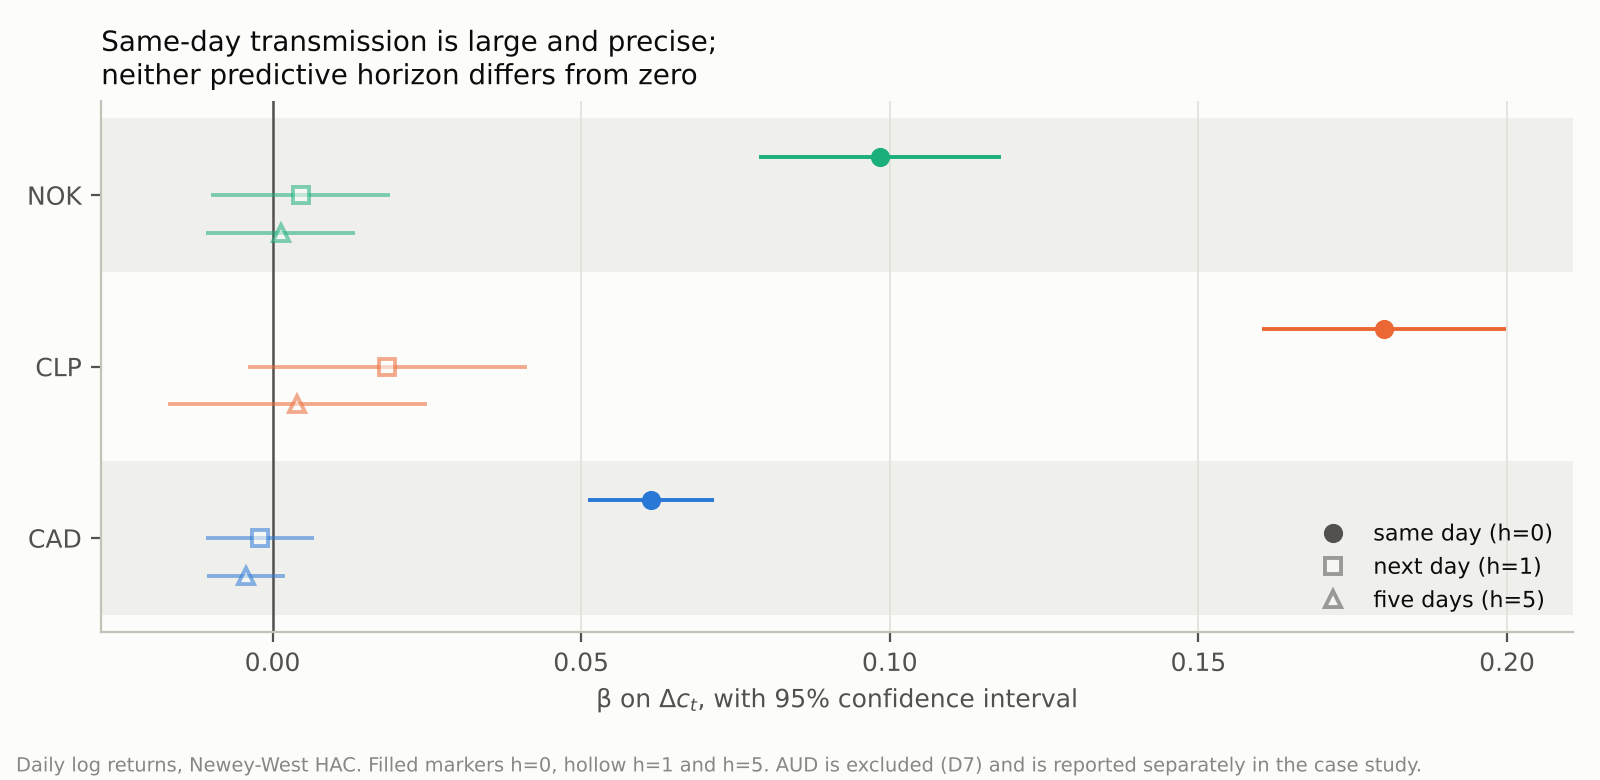
\includegraphics[width=0.92\textwidth]{fig6_coefficients.png}
\caption{Coefficients with 95\% confidence intervals at all three horizons. The
same-day estimates sit far from zero with tight intervals; both predictive
horizons straddle it.}
\end{figure}

\begin{figure}[htbp]
\centering
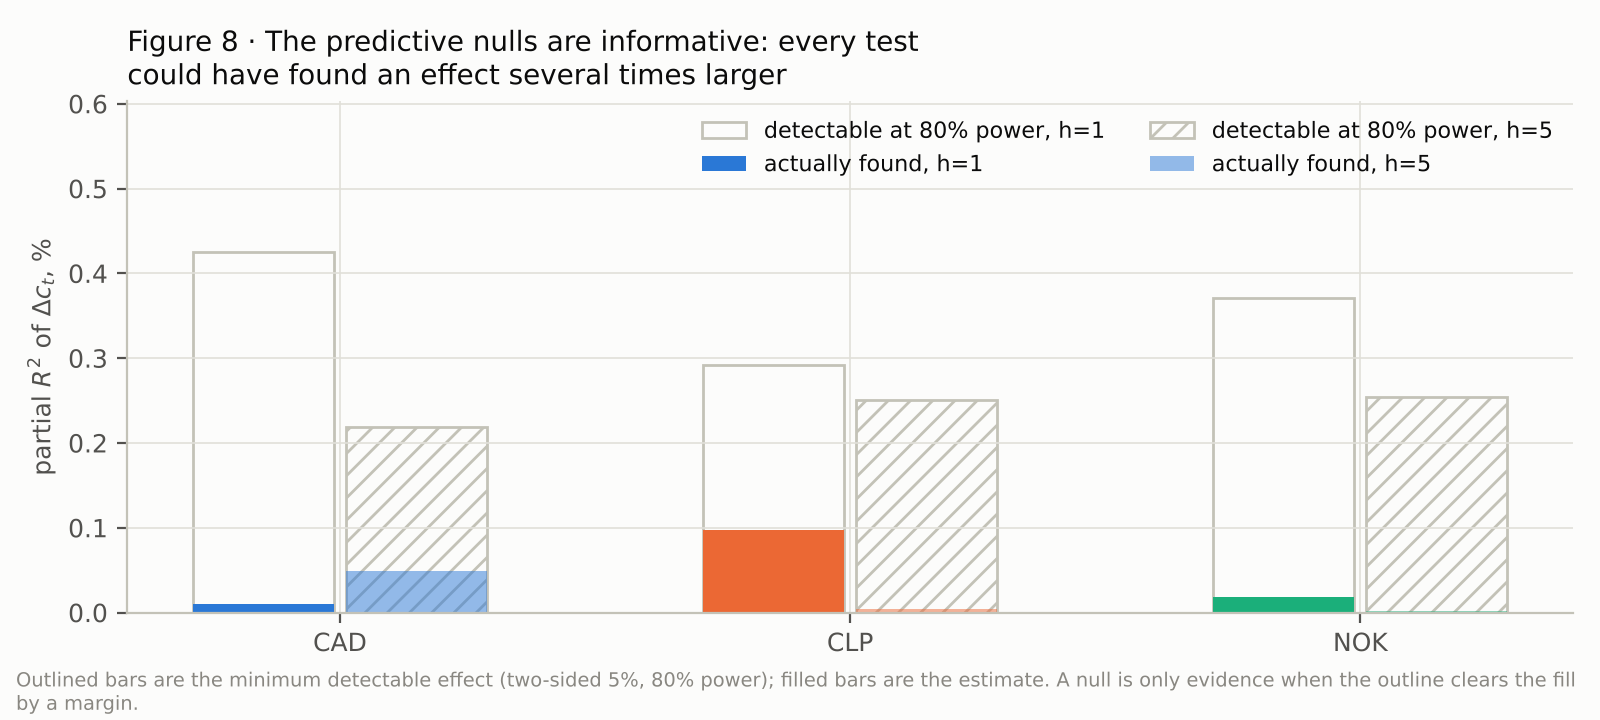
\includegraphics[width=0.92\textwidth]{fig8_power.png}
\caption{Minimum detectable effect against the estimate actually obtained. A
null is evidence only when the outlined bar clears the filled one by a margin,
which it does at both predictive horizons for all three pairs.}
\end{figure}

\begin{figure}[htbp]
\centering
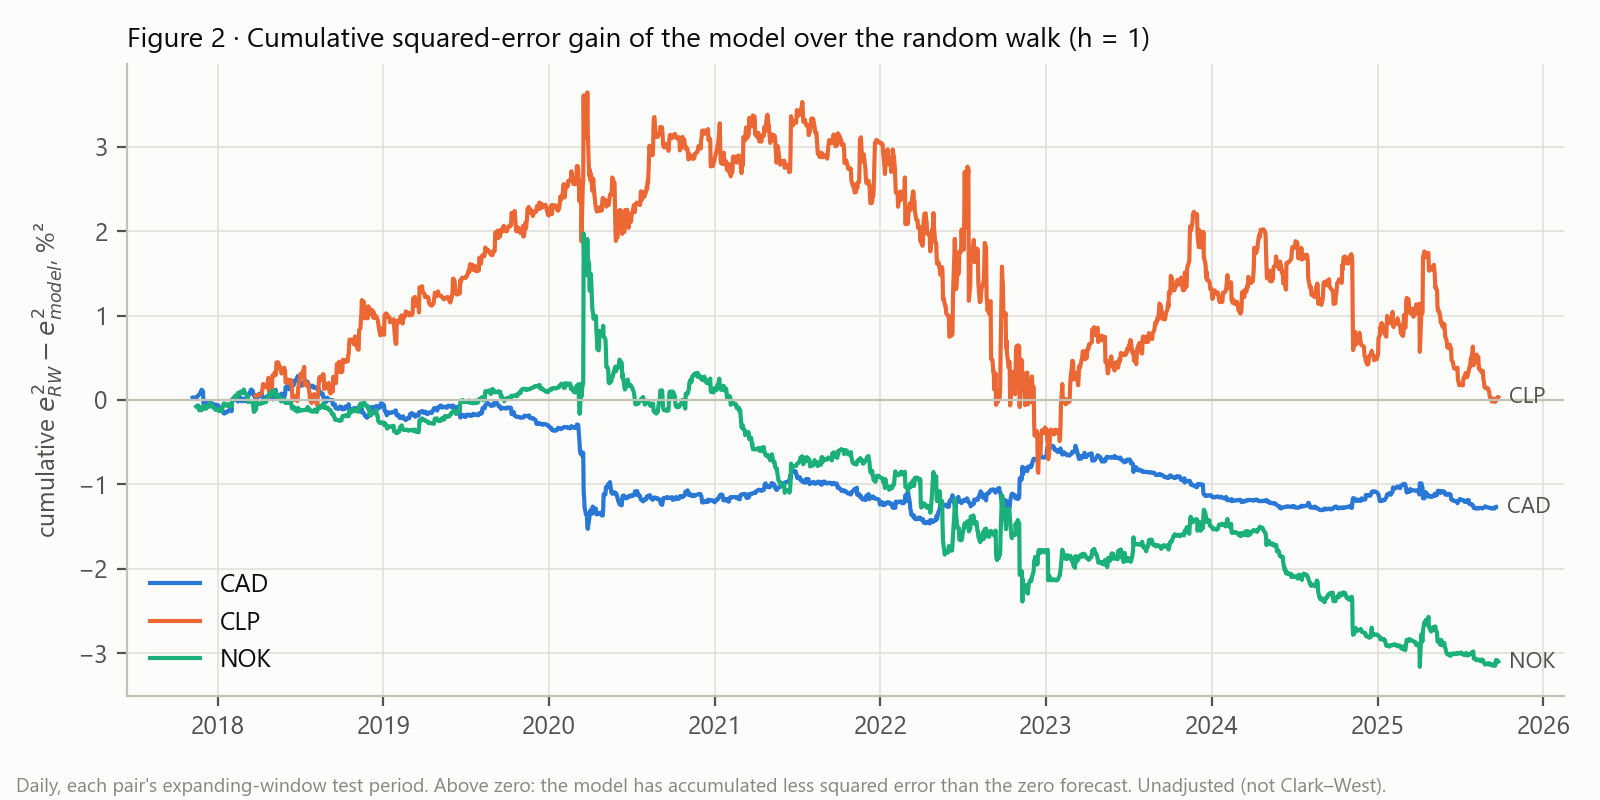
\includegraphics[width=0.9\textwidth]{fig2_cumulative_loss.png}
\caption{Cumulative squared-error loss differential against the random walk.
A persistently rising line would indicate genuine predictive gain; none is
present at either horizon for any pair.}
\end{figure}

\begin{figure}[htbp]
\centering
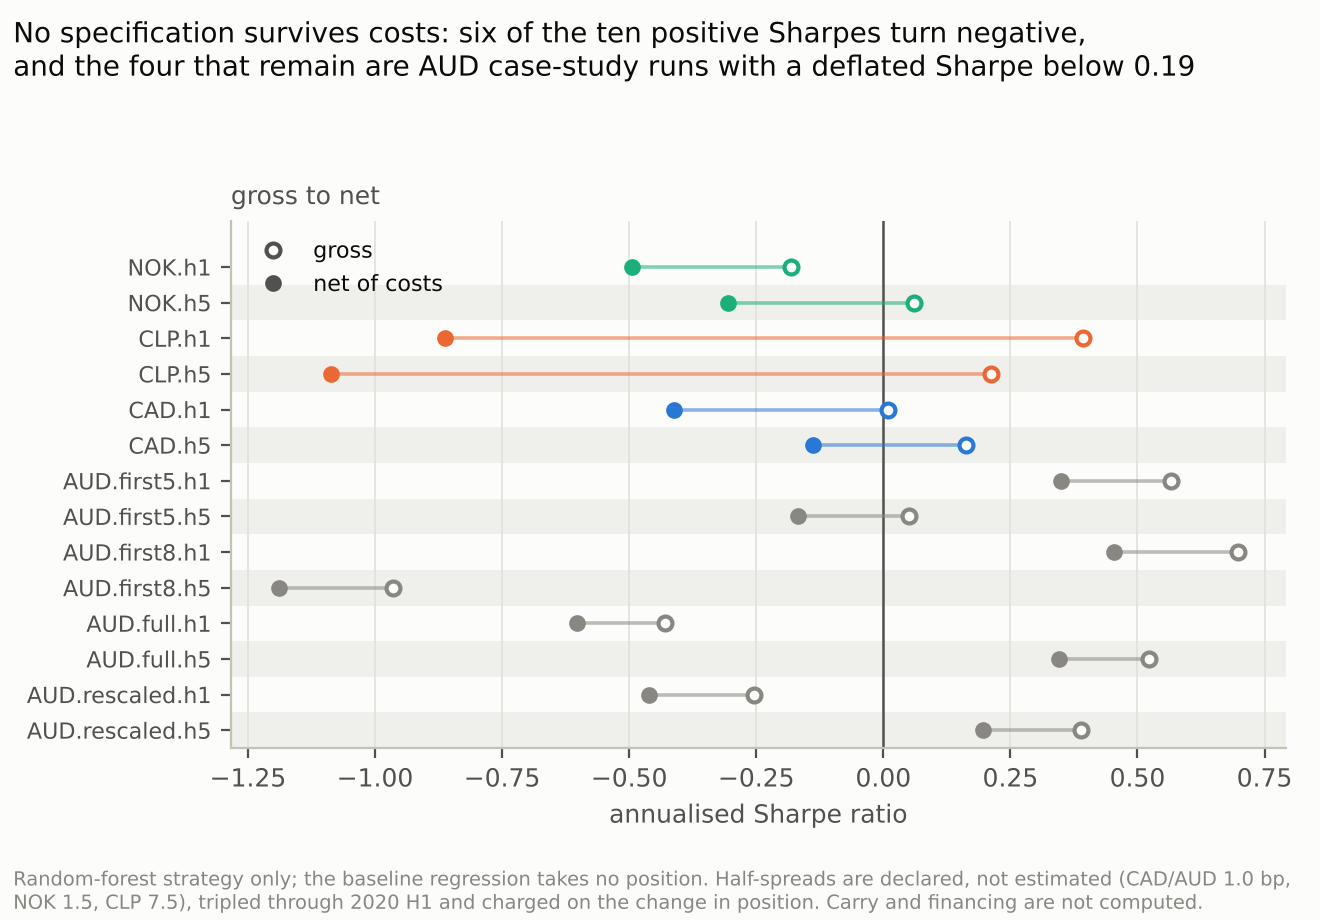
\includegraphics[width=0.96\textwidth]{fig9_costs.png}
\caption{Costs on the random-forest strategy, by specification: the move from
gross Sharpe (hollow) to net (filled). A line crossing the zero rule marks a
strategy that only made money before paying for itself. The four that stay
positive are all AUD case-study specifications, and none of them clears a
deflated Sharpe of 0.95.}
\end{figure}

\subsection{The placebo fails, and this is the principal limitation}
\label{sec:placebo}

Two non-commodity currencies were used as negative controls. Neither
Switzerland nor the United Kingdom exports these commodities, so neither should
respond to them once the dollar is controlled. Both do.

\begin{table}[htbp]
\centering
\caption{Placebo outcomes, $h=0$}
\begin{tabular}{lrrr}
\toprule
 & CAD & CLP & NOK \\
\midrule
Commodity currency $\beta$ & $+0.0613$ & $+0.1800$ & $+0.0984$ \\
\textbf{GBP placebo}       & $\mathbf{+0.0158}$ & $\mathbf{+0.0269}$ & $\mathbf{+0.0193}$ \\
\textbf{CHF placebo}       & $\mathbf{-0.0198}$ & $-0.0157$ & $\mathbf{-0.0209}$ \\
\midrule
GBP $p$ & $<0.001$ & $<0.001$ & $<0.001$ \\
CHF $p$ & $<0.001$ & $0.052$  & $<0.001$ \\
\bottomrule
\end{tabular}
\end{table}

The pattern is a \textbf{risk-appetite factor the dollar control does not
absorb}: risk-on lifts commodities and commodity currencies strongly, lifts a
cyclical non-commodity currency weakly, and weakens the canonical safe haven.
Sterling loads positive because it shares the factor; the franc loads negative
because it mirrors it. The franc alone would have been a poor control for
exactly this reason, which is why sterling was added.

Taking the sterling loading as the generic cyclical-currency response, the
common factor accounts for roughly \textbf{26\% of the CAD coefficient, 15\% of
CLP's and 20\% of NOK's}. The remainder is plausibly commodity-specific, and the
sign, significance and ordering of the three pairs are unaffected. But the
contemporaneous result cannot be read as a pure terms-of-trade effect, and it is
not reported as one here.

The predictive null is untouched: a common contemporaneous factor does not
create forecastability, and none is found.

\begin{figure}[htbp]
\centering
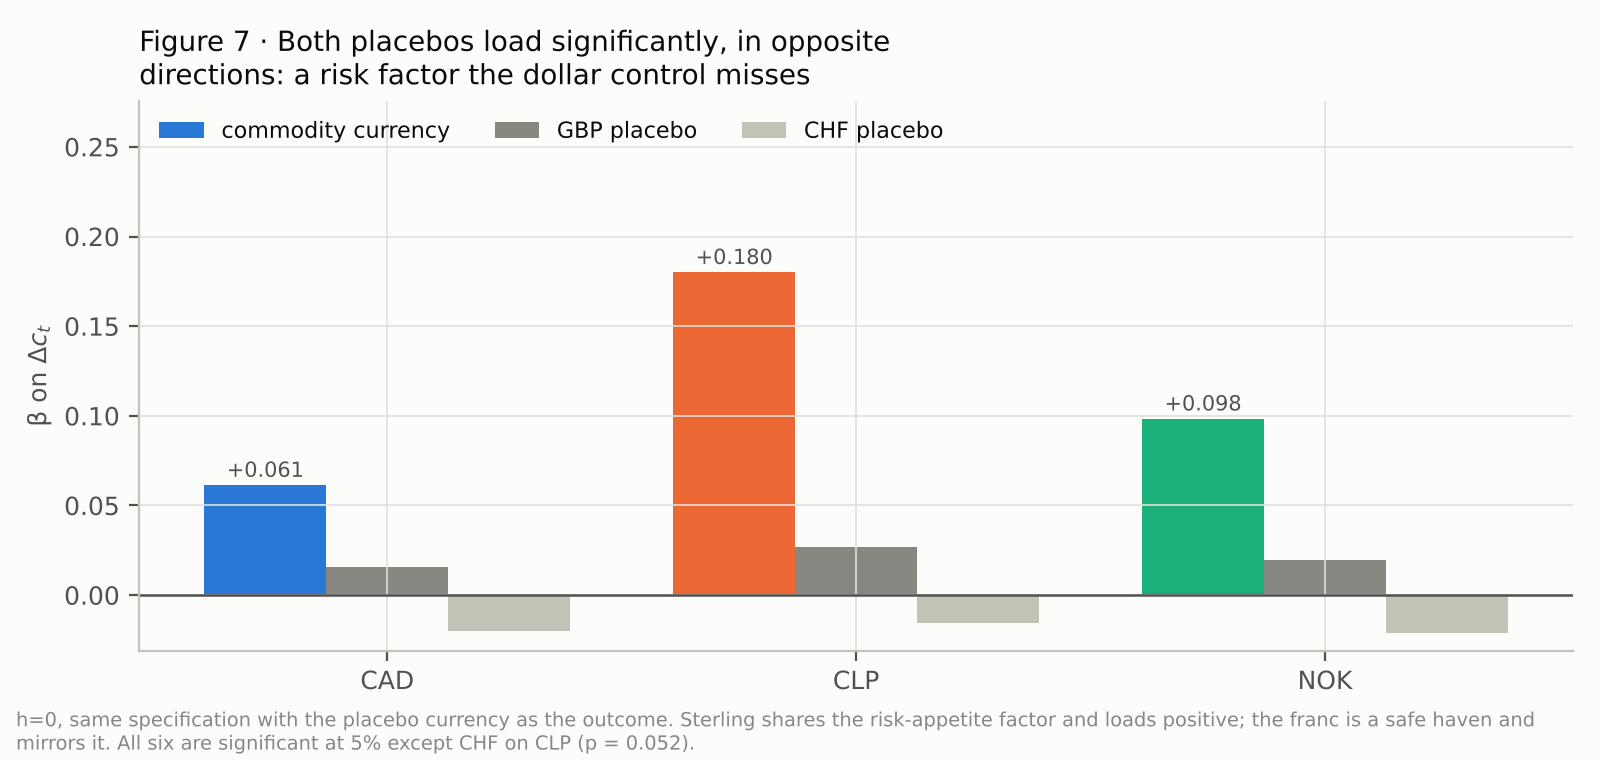
\includegraphics[width=0.92\textwidth]{fig7_placebo.png}
\caption{Placebo loadings beside the commodity-currency coefficients. Sterling
shares the risk-appetite factor and loads positive; the franc is a safe haven
and mirrors it. Both are an order of magnitude smaller than the effect of
interest.}
\end{figure}

\section{Robustness}

Table~4 of the output set reports every prespecified check. Nothing overturns
the headline results; three are worth noting.

\textbf{The dollar control matters most for CLP.} Replacing ICE DXY with the Fed
broad dollar index moves the CLP coefficient from $0.180$ to $0.114$, the
largest sensitivity anywhere in the study. The Fed index is weighted toward
trading partners including China, so it plausibly absorbs part of the Chinese
demand factor that drives copper. The other pairs barely move.

\textbf{CAD is a DXY constituent.} The dollar control contains the dependent
variable at 9.1\% weight for that pair alone. A dollar index rebuilt without CAD
from its remaining components (covering 86.7\% of the non-CAD basket; SEK
unavailable) correlates $0.953$ with the full index and leaves the coefficient
essentially unchanged.

\textbf{The WTI source question closed empirically.} Two library files disagreed
on one date. Retrieving the alternative showed the two are \textbf{identical on
3{,}960 of 3{,}961 overlapping dates}, differing only on 23 September 2025 by
$0.28$. Re-estimating CAD on the alternative reproduces the coefficients to four
decimal places.

Also run without material effect: BCOM orthogonalized on LME rather than COMEX
copper; NOK restricted to pre-2022, when Brent still represented Norwegian
export revenue before gas became comparable; long-span Chilean returns retained
with a span control; indeterminate-roll Brent observations retained; 2020~H1
dropped; the largest commodity move dropped per pair.

One check could not be run: the AUD zero-return diagnostic, because the frozen
specification defined its trigger (``if AUD proves unstable at the sample
start'') without an operational rule. That is recorded as an omission rather
than quietly dropped.

\section{AUD and iron ore: a case study in instrument choice}
\label{sec:aud}

AUD is reported separately and is not part of the cross-pair comparison. The
reason is not that it gives an inconvenient answer but that its regressor is
measured differently from the other three in a way that is derivable in advance.

\subsection{The mechanism}

The SGX contract settles against the \textbf{arithmetic average} of all IODEX
62\% Fe prints in the expiring month. With $N$ prints in the month and $k$
elapsed, a shock to today's index enters the realized portion at weight $1/N$
and the forecast of the remaining prints at weight $(N-k)/N$, so under a random
walk the pass-through from index to futures is

\begin{equation}
w_k \;=\; \frac{N-k+1}{N}
\label{eq:w}
\end{equation}

falling from approximately 1 on the first day to $1/N$ by the last. The data
agrees: mean absolute daily return falls from $1.36\%$ on day 2 to $0.17\%$ on
day 21, while WTI and Brent remain flat at $1$--$2\%$ throughout their contract
months.

\begin{figure}[htbp]
\centering
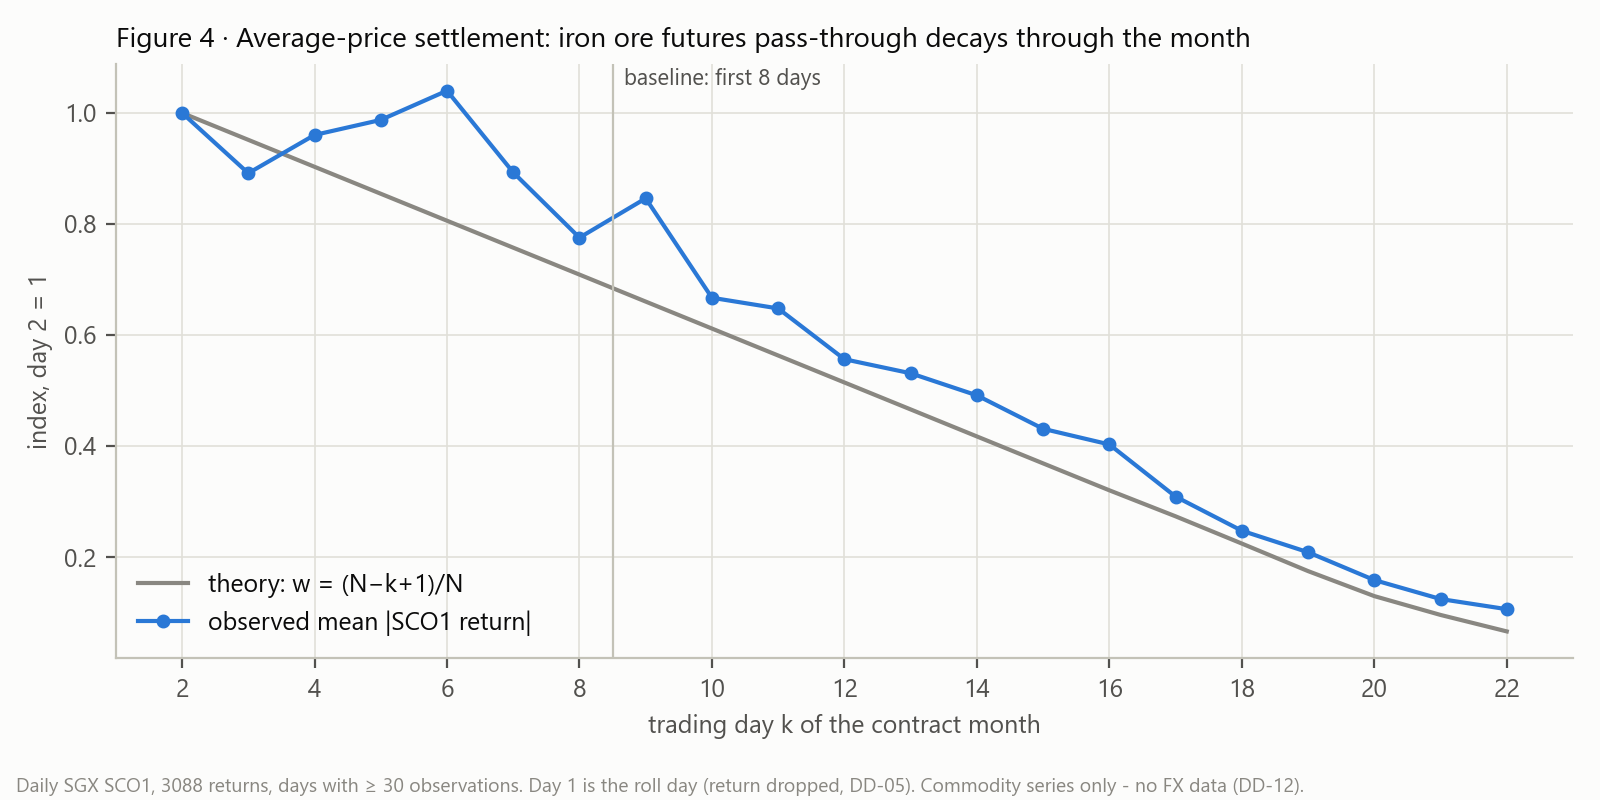
\includegraphics[width=0.85\textwidth]{fig4_iron_ore_decay.png}
\caption{Mean absolute daily return by trading day within the contract month.
Iron ore decays monotonically, consistent with \eqref{eq:w}; crude does not.}
\end{figure}

A second property compounds it. Agency assessments are sticky, since values
are carried forward when physical liquidity is thin, and iron ore is the only
commodity in the study with \textbf{positive} first-order autocorrelation.

\begin{table}[htbp]
\centering
\caption{First-order autocorrelation of commodity log returns}
\begin{tabular}{lrrr}
\toprule
Series & AC(1) & $t$ & Zero-return days \\
\midrule
Iron ore & $\mathbf{+0.046}$ & $+2.57$ & $\mathbf{2.12\%}$ \\
WTI      & $-0.033$ & $-2.03$ & $0.42\%$ \\
Brent    & $-0.006$ & $-0.39$ & $0.25\%$ \\
Copper   & $-0.031$ & $-1.99$ & $0.89\%$ \\
\bottomrule
\end{tabular}
\end{table}

Crude and copper show the slight negative autocorrelation characteristic of
bid--ask bounce. A positively autocorrelated regressor manufactures a lead--lag
artifact, and AUD is the one pair that fails the date-shift alignment test: its
coefficient at a one-day backward shift ($+0.0227$, $t=2.51$) \emph{exceeds} its
contemporaneous coefficient ($+0.0166$). The two symptoms share one cause.

\subsection{The correction does not rescue the pair}

\begin{table}[htbp]
\centering
\caption{AUD under four treatments of the iron ore regressor}
\begin{tabular}{lrrr}
\toprule
Treatment & $\beta$ & $p$ & $N$ \\
\midrule
Full sample                      & $+0.0166$ & $0.016$ & 2{,}963 \\
First 8 days of contract month   & $+0.0166$ & $0.037$ & 1{,}023 \\
First 5 days                     & $+0.0125$ & $0.235$ & 575 \\
\textbf{Rescaled by $1/w$}       & $\mathbf{+0.0075}$ & $0.047$ & 2{,}963 \\
\bottomrule
\end{tabular}
\end{table}

The rescaling behaves exactly as the algebra predicts, which confirms the
correction is working. But it puts the attenuation-corrected coefficient at
roughly $0.0075$, against $0.061$ for CAD and $0.180$ for CLP, an order of
magnitude below rather than comparable.

\textbf{So the measurement problem is real, documented, and not what makes AUD
weak.} Two explanations remain and neither is tested here. The first is timing:
on published and conventional settlement times, iron ore settles approximately
10.5 hours before the FX snap, against 2.5 hours for the oil pairs, and the gap moves on 37.8\% of days because Singapore
observes no daylight saving while New York does. The same-day AUD observation
therefore contains most of a trading day \emph{after} the commodity print. The
second is simply that iron ore transmits less strongly to AUD than oil does to
CAD and NOK or copper does to CLP, which is plausible given that coal is
comparable to iron ore in the Australian export basket.

The useful result here is a negative one about method: a correction derived from
first principles, applied correctly, and found not to explain the anomaly it was
built for.

\section{Limitations}

Stated in descending order of how much they constrain the conclusions.

\begin{enumerate}\itemsep2pt
\item \textbf{The placebo failure} (\S\ref{sec:placebo}). A risk-appetite factor
the dollar control does not absorb accounts for roughly $15$--$26\%$ of the
contemporaneous coefficients. The same-day result is not a pure terms-of-trade
estimate.
\item \textbf{AUD carries two independent measurement problems} and is excluded
from the comparison for that reason, leaving a three-pair rather than four-pair
test.
\item \textbf{The sample ends September 2025}, three months short of the
requested window, because of inherited file coverage.
\item \textbf{The Chilean peso has a 2012 coverage hole} of 121 missing
weekdays; 18 returns were excluded for spanning more than five calendar days.
\item \textbf{The iron ore ticker was recovered from returned contract codes},
not confirmed on the terminal.
\item \textbf{No volume or open-interest data} was obtainable, so
early-contract liquidity could not be verified.
\item \textbf{Bloomberg Desktop API access was suspended}, which prevented the
sample extension.
\item \textbf{$h=5$ is the single-day return five days ahead}, as the frozen
equation defines it, not a cumulative five-day return. The cumulative version
was not tested.
\end{enumerate}

\section{Conclusion}

The contemporaneous-strong, predictively-weak pattern generalizes. Across CAD,
CLP and NOK, a one-standard-deviation commodity move corresponds to between
$+0.154\%$ and $+0.240\%$ of same-day currency appreciation, significant beyond
any conventional threshold after controlling for broad dollar and broad
commodity moves and after Holm adjustment. None of the three forecasts the next
day, and the nulls are informative rather than merely quiet: the tests could
have detected effects several times larger than those observed, no pair beats a
random walk out of sample, and a nonlinear learner finds nothing the linear
model missed.

Two qualifications carry real weight. The first is that a risk-appetite factor
survives the dollar control and accounts for perhaps a fifth of the
contemporaneous relationship, so the same-day finding is not purely a
terms-of-trade effect. The second is the fourth pair: AUD could not be included,
because the only available iron ore instrument settles against a monthly average
of a smoothed index, and correcting for that, which can be done and was, leaves
the coefficient an order of magnitude below the others rather than in line with
them.

That second qualification may be the more transferable finding. A literature
built on commodity-currency transmission takes the commodity price series as
given. For iron ore there is no unattenuated traded instrument: every cleared
contract settles on a monthly average, because that is how the physical market
contracts. Any study including AUD inherits that, whether or not it says so.

\section*{References}
\begin{list}{}{\leftmargin=1.5em \itemindent=-1.5em \itemsep3pt}

\item Bailey, D.~H. and M. L\'opez de Prado (2014). The deflated Sharpe ratio:
correcting for selection bias, backtest overfitting, and non-normality.
\emph{Journal of Portfolio Management} 40(5), 94--107.

\item Cameron, A.~C., J.~B. Gelbach and D.~L. Miller (2011). Robust inference
with multiway clustering. \emph{Journal of Business and Economic Statistics}
29(2), 238--249.

\item Chen, Y., K. Rogoff and B. Rossi (2010). Can exchange rates forecast
commodity prices? \emph{Quarterly Journal of Economics} 125(3), 1145--1194.

\item Clark, T.~E. and K.~D. West (2007). Approximately normal tests for equal
predictive accuracy in nested models. \emph{Journal of Econometrics} 138(1),
291--311.

\item Driscoll, J.~C. and A.~C. Kraay (1998). Consistent covariance matrix
estimation with spatially dependent panel data. \emph{Review of Economics and
Statistics} 80(4), 549--560.

\item Ferraro, D., K. Rogoff and B. Rossi (2015). Can oil prices forecast
exchange rates? An empirical analysis of the relationship between commodity
prices and exchange rates. \emph{Journal of International Money and Finance}
54, 116--141.

\item Holm, S. (1979). A simple sequentially rejective multiple test procedure.
\emph{Scandinavian Journal of Statistics} 6(2), 65--70.

\item Newey, W.~K. and K.~D. West (1994). Automatic lag selection in covariance
matrix estimation. \emph{Review of Economic Studies} 61(4), 631--653.

\end{list}

\section*{Reproducibility}

\begin{table}[htbp]
\centering
\small
\begin{tabular}{ll}
\toprule
Specification freeze     & 26 October 2026, hashes in \texttt{FREEZE.md} \\
Decisions and amendments & \texttt{design\_decisions.md} (D1--D7) \\
Source provenance        & \texttt{manifests/source\_inventory.csv}, \texttt{bloomberg\_source\_log.csv} \\
Variable definitions     & \texttt{manifests/variable\_dictionary.csv} \\
Sample attrition         & \texttt{manifests/sample\_attrition.csv} \\
Forecast origins         & \texttt{manifests/forecast\_origins.csv} \\
Machine-readable results & \texttt{outputs/tables/results\_primary.csv}, \texttt{results\_robustness.csv}, \texttt{results\_rf\_dsr.csv}, \texttt{results\_costs.csv} \\
Seed                     & 20261026 \\
Rebuild                  & \texttt{src/00} $\to$ \texttt{01} $\to$ \texttt{03} $\to$ \texttt{04} $\to$ \texttt{05} $\to$ \texttt{06} $\to$ \texttt{07} $\to$ \texttt{08} $\to$ \texttt{08b} $\to$ \texttt{08c} $\to$ \texttt{09} \\
\bottomrule
\end{tabular}
\end{table}

Every table and figure in this paper is generated by
\texttt{src/09\_tables\_figures.py} from the saved results tables. None was
edited by hand.

\end{document}
